\linespread{1.13}\selectfont

%%%%%%%%%%%%%%%%%%%%%%%%%%%%%%%%%%%%%%%%%%%%%%%%%%%%%%%%%%%%%%%%%%
%%%%%%%%%%%%%%%%%%%%%%%%%%%%%%%%%%%%%%%%%%%%%%%%%%%%%%%%%%%%%%%%%%
\chapter{Создание сервиса прогнозирования}
%%%%%%%%%%%%%%%%%%%%%%%%%%%%%%%%%%%%%%%%%%%%%%%%%%%%%%%%%%%%%%%%%%
%%%%%%%%%%%%%%%%%%%%%%%%%%%%%%%%%%%%%%%%%%%%%%%%%%%%%%%%%%%%%%%%%%
\section{Подготовка инструментов}
Необходимо установить IDE NetBeans, при установке указать что требуется установить сервер приложений GlassFish. Его можно заменить на аналоги, например Wildfly.  

Для начала необходимо создать новый java проект в IDE (Через меню: Файл -> создать проект или нажатием кнопки на тулбаре), и указать что он будет web приложением (рис. \ref{pict:projecttype}). Создание такого типа приложения позволит строить распределенную систему из отдельных компонент без привязки к физическому расположению. 

\begin{figure}[h!]
\center
	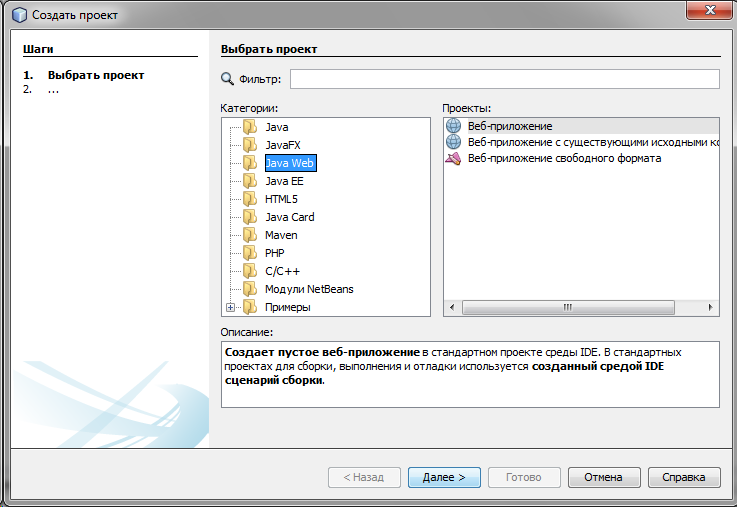
\includegraphics[width=450px]{service/1.png}
	\caption{Тип проекта}
	\label{pict:projecttype}
\end{figure}

Задаем наименование проекта, указываем его расположение (рис. \ref{pict:projectname}). Проект, созданный по данной инструкции будет использовать ant в качестве системы управления сборкой. 

\begin{figure}[h!]
\center
	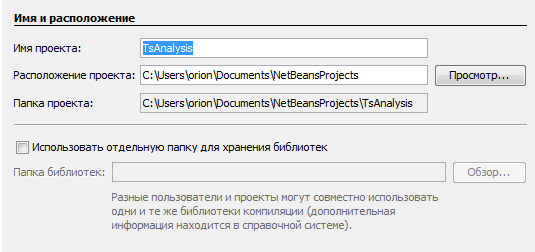
\includegraphics[width=450px]{service/2.png}
	\caption{Название проекта}
	\label{pict:projectname}
\end{figure}

Далее нужно указать IDE, на какой сервер будет разворачиваться приложение (рис. \ref{pict:projectserv}). Эта настройка позволят запускать приложение напрямую из IDE. Разумеется, если приложение впоследствии будет, развернуто на другом сервере то настройки указанные здесь никак не помешают этому. Здесь следует сделать замечание, что по умолчанию будет выбран сервер, который был установлен вместе с IDE. Поэтому если используется другой сервер приложений, то его потребуется сначала добавить, т.е. сделать доступным для выбора. Процедура выбора заключается в указании каталога размещения нового сервера. 

Контекстный путь - это путь, по которому можно получить доступ к приложению после его развертывания на сервере, например:
\begin{verbatim}
	http://localhost:8080/TsAnalysis
\end{verbatim}

\begin{figure}[h!]
\center
	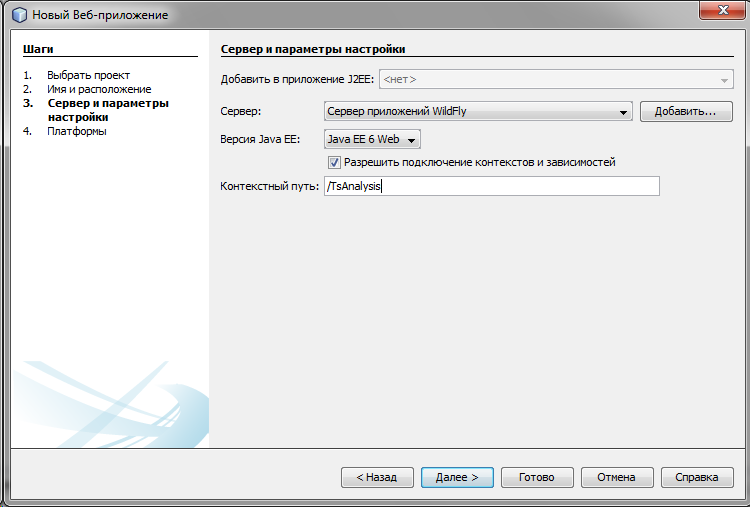
\includegraphics[width=450px]{service/3.png}
	\caption{Выбор сервера}
	\label{pict:projectserv}
\end{figure}

После прохождения последних шагов, в которых нужно все оставить по умолчанию будет сформировано дерево проекта и открыта стартовая страница приложения (рис. \ref{pict:projecttree}). 

В подкаталоге проекта "Веб страницы" расположены *.jsp файлы,являющиеся страницами Java Server Pages. Технология JSP предназначена для создания содержимого страницы из статического и динамического контента. Для создания web-сервиса данный функционал не потребуется.

Подкаталог "Пакеты исходных кодов" содержит файлы с определением классов реализуемой системы. Пакетом (package) в java называется механизм, позволяющий располагать классы в пространстве имен, тем самым формируя подобие модульной структуры.

\begin{figure}[h!]
\center
	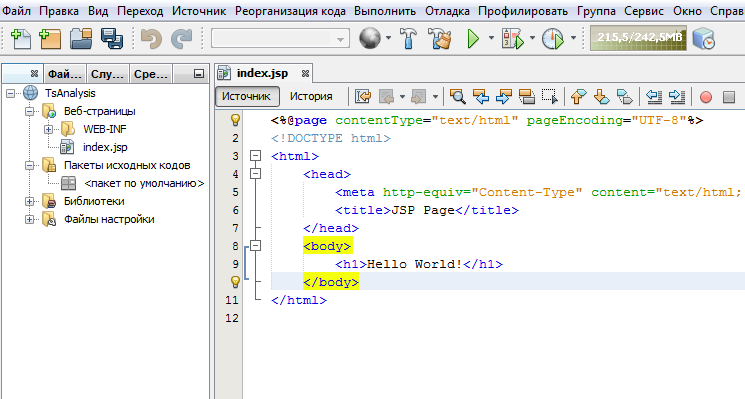
\includegraphics[width=450px]{service/5.png}
	\caption{Структура проекта}
	\label{pict:projecttree}
\end{figure}



